\input sys/inputs.tex
\usepackage[czech]{babel}

\begin{document}

\bigheading{Protikouzla}

% \info{task_name}{infile}{outfile}{points}{timelimit}{memlimit}
% leave this values, if you are not interested
\info{counterspells}{stdin}{stdout}{100}{1000 ms}{1 GB}

Karetní hra \emph{Magic: The Gathering} má zajímavý herní mechanizmus
kouzel a protikouzel. Nebudeme jej zde vysvětlovat, jelikož je poměrně
složitý a k vyřešení této úlohy jej není nutné znát. Pokud ovšem znáte MTG,
jistě si uvědomíte, jak tato úloha souvisí s mechanizmem protikouzel.

\heading{Úloha}

Pro každý zakořeněný strom existuje právě jeden způsob, jak obarvit jeho vrcholy
dvěma barvami (černou a bílou) tak, aby byla pro každý vrchol splněna následující podmínka:
\begin{itemize}
\item Vrchol je bílý, právě když má alespoň jednoho černého syna.
\end{itemize}

Takto obarvený strom budeme nazývat \emph{dobře obarvený}.
Jednoznačnost takového obarvení lze jednoduše dokázat indukcí.
Zejména si uvědomte, že podmínka vynucuje rovněž to, že každý list je černý.


Začneme se zakořeněným stromem sestávajícím z jediného (černého) vrcholu
a $n$-krát provedeme následující operaci:

\begin{itemize}
\item $add(v)$ -- Přidej nový černý vrchol jako syna vrcholu $v$. Poté přebarvi některé
                  (možná žádný, možná všechny) vrcholy stromu tak, aby byl opět dobře obarvený.
\end{itemize}

Po každé operaci chceme vědět, kolik vrcholů muselo být přebarveno.

\heading{Vstup}

Kořen stromu má číslo $0$. Další vrcholy mají čísla $1, 2, \dots, n$
podle pořadí, v němž byly přidávány.

První řádek vstupu obsahuje celé číslo $n$ ($1 \leq n \leq 200000$) -- 
počet operací (přidaných vrcholů).

Následuje $n$ řádků, z nichž $i$-tý obsahuje celé číslo $v_i$ -- číslo otce vrcholu,
který byl přidán v $i$-té operaci. Můžete předpokládat, že vrchol $v_i$ již existuje před $i$-tou operací,
tedy že $v_i < i$.

\heading{Výstup}

Za každou operaci vypište jeden řádek a na něm počet vrcholů,
které musely být při této operaci přebarveny.

\heading{Podproblémy}

\centering
\begin{tabular}{|l|l|l|l|}
\hline
podproblém & body & nejvyšší $n$ & další omezení                  \\ \hline
1       & 20     & 1000      &                                        \\ \hline
2       & 20     & 10000     &                                        \\ \hline
3       & 20     & 100000     &                                        \\ \hline
4       & 20     & 200000    & hloubka výsledného stromu je nejvýš 100 \\ \hline
5       & 20     & 200000    &                                        \\ \hline
\end{tabular}

\heading{Příklady}


\sampleIN
5
0
1
2
1
3
\sampleOUT
1
2
3
2
2
\sampleCOMMENT
Jak vypadá strom po jednotlivých operacích, je znázorněno níže
(přebarvené vrcholy jsou zvýrazněny):
\sampleEND
\center{
\includegraphics[width=12cm]{img/counterspells}
}
\end{document}
